\documentclass[10pt]{article}
\usepackage{titling}
\usepackage[margin=0.75in]{geometry}
\usepackage{graphicx}
\graphicspath{ {images/}}
\title{Requirements Document}
\author{
	Dylan Davis, Trevor Hammock, Alex Schultz \\
	Oregon State University\\
	Corvallis, Oregon
}
\date{\today}

\begin{document}
\begin{titlingpage}
\maketitle

\begin{abstract}

HP's PageWide Web Press division develops and troubleshoots their industrial web presses. These web presses send over 350GB a day of business analytics and product issues. This has caused a storage/performance dilemma for their team's back-end Database. To solve this my group will research and test various compression options available for Oracle Databases. Once we have gathered the necessary data, we will then propose and implement a solution for the current Database. After that has taken place we will then compile all of our findings into a report and submit that to a Oracle Performance Tuning conference in the Spring.

\end{abstract}
\end{titlingpage}


\tableofcontents
\clearpage


\section{Introduction}
\subsection{Purpose}

PageWide Web Press, a printing division within HP, produces and supports industrial digital web presses. All of the web presses currently deployed out in the market generate product data which the PageWide Web Press team receives on a daily basis. The data is eventually stored into a Oracle Database and is used to perform business analytics or resolve product issues for the web presses.

However this data is currently creating a plethora of issues for the division. On average the division receives around 350GB of product data per day which generates Database tables with over billions of rows. This massive influx of data has stressed the division's storage and performance capabilities of their current hardware. This significantly increases the amount time it takes to process and analyze that data on top of making more difficult to store. Additionally the amount of data that is received everyday has slowly been increasing over time. What could be 350GB of data per day today could be 450 to 500 GB of data tomorrow.

If nothing is done about the data collection, the division may need make a costly investment into better hardware that can meet their growing storage and performance needs. Or they might have to invest into big data software platforms, like Hadoop, that are more optimized and scalable for their given workloads. This project will address this issue by using system enabled compression to reduce the amount of physical space that the data occupies as a means to mitigate the storage and performance issues.


\subsection{Scope}

What this project will do is investigate various compression options that Oracle provides for their Database systems and use that information to implement a solution for PageWide Web Press's storage crisis. This project will not alter or restructure the data itself but rather change how the Database system stores said data into the physical storage medium. This project for the most part will not actively look into or investigate query performance options for this solution (like Oracle's in-memory compression for example...citation).

Essentially the goal of this project is to address the division's data issues by using compression to reduce the amount of space that the data occupies. If implemented properly compression should help delay a costly hardware/software upgrade for their storage needs and hopefully improve the query performance for their Database system.


\subsection{Definitions, acronyms, and abbreviations}


HP: Stands for Hewlett-Packard which is a multinational IT company that is infamous for their printing products.\\
PageWide Web Press: A printing division within HP that develops and supports HP's industrial digital web presses.\\
Database: A structured set of data that primarily used/optimized in web based environments.\\
Query: In Databases it is a request that processes and/or returns data from within a Database.\\
Oracle: A multinational IT company that specializes in enterprise solutions such as Database software or cloud systems.\\
Oracle Database: A relational Database system that is produced and supported by Oracle.\\
Hadoop: A software framework that is optimized and designed for processing of big data.\\
Block: In Oracle Database it is a specific number of bytes that holds data within a Database. The size is typically fixed and as much data is stuffed into a block as possible before it is stored onto the physical storage medium.\\
Oracle Linux: A distribution of Linux that is maintained by Oracle. It is optimized platform for many of their products, such as Oracle Database.\\
RMAN\\
I/O: Stands for input and output. Typically associated with the rate or usage of how data is read or written to a physical storage medium.


\subsection{References}
\subsection{Overview}


\section{Overall Description}
\subsection{Product perspective}
\subsection{Product functions}
\subsection{User characteristics}
\subsection{Constraints}

\begin{itemize}
	\item Only compression options available in Oracle Database 12.2 will be examined.
	\item System characteristics and properties will also be examined. An example of this will be looking into the effect that block size has on the compression algorithms.
	\item Compression options that have stricter licensing or hardware dependencies will be ignored.
	\item The data and how it is structured will be left intact. However how that data gets stored into the physical storage medium will change.
	\item Data properties and characteristics will also be examined. Which will include:
		\begin{itemize}
			\item How the columns are ordered
			\item The cardinality
			\item Repetition within the datasets
		\end{itemize}
	\item Compression options that show little to no benefits will be ignored for the final implementation.
\end{itemize}


\subsection{Assumptions and dependencies}

\begin{itemize}
	\item It is assumed that all of Databases used in this project will be installed on a distribution of Oracle Linux 7.
	\item It is assumed that all of Oracle Databases used in this project will be version 12.2
	\item It is assumed that the system performing the benchmarks for this project can record system statistics, such as CPU usage, within a reasonable time resolution.
\end{itemize}

\subsection{Apportioning of requirements}

If time permits the following stretch goals may be looked at:
\begin{itemize}
	\item Enabling Oracle's new Network Compression (citation) and see the effect it has network bandwidth.
	\item Researching and/or playing with Oracle's Advanced Index Compression (citation) to investigate additional space/performance savings.
	\item Oracle's Backup Compression (RMAN) (citation) to address future storage issues with their regularly scheduled backups.
\end{itemize}

\section{Requirements}
\begin{itemize}
	\item For this project all of tests and analysis will be performed on systems/data that mirror PageWide Web Press's current environment.
	\item That the students conducting this project will learn about and reverse engineer a data block in Oracle to understand how the data gets stored.
	\item That the Oracle compression algorithms that will be tested for this project are reversed engineer (to the best that can be inferred) to understand how it interacts with a set of data.
	\item Once the background research is done, the students conducting this project will then design a set of experiments to prove/test the findings they found during the research phase.
	\item For the experiments the students will create and use a set of scripts that will track critical system information such as CPU, I/O, or Memory usage.
	\item Once all of the data from the experiments is collected, it will be compiled into a white paper that will summarize the research and findings of this project.
	\item Finally that white paper will be presented at an Oracle Database conference in the Spring.
	\item Then the students for the remainder of the project will design and possibly integrate a solution into PageWide Web Press's current environment.
\end{itemize}
Here is our Gantt Chart outlining the tasks and tentative due dates: \\
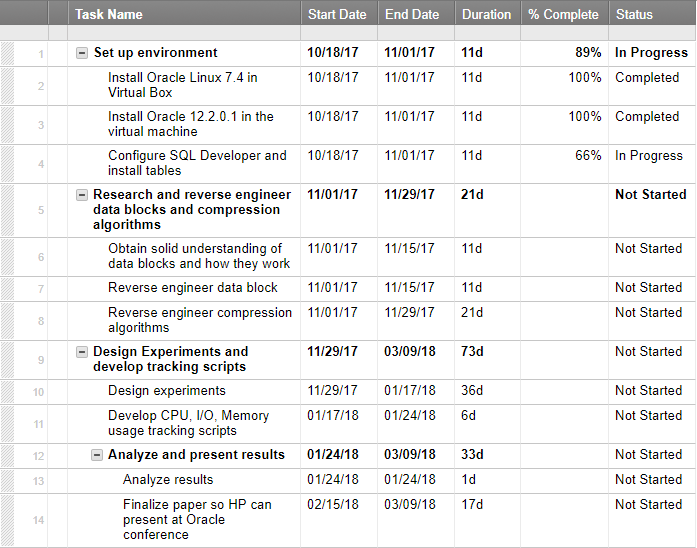
\includegraphics{gantt.png}


\end{document}